\documentclass[oneside]{tietreport}

% Prevent blank pages inserted before chapters (keep chapters on the next available page).
\makeatletter
\@openrightfalse
\makeatother

% Import images
\usepackage{graphicx}
\usepackage{needspace}
\usepackage{float}
\usepackage{placeins}

% Test case tables
\usepackage{array}
\usepackage{tabularx}

% Bibliography configuration
\usepackage[
  date=year,
  style=alphabetic,
  backend=biber,
  sorting=nty,
  maxnames=5,
  minnames=3,
  maxalphanames=4,
  minalphanames=3,
  backref=true,
  doi=false,
  isbn=false,
  url=false,
  eprint=false
]{biblatex}
\addbibresource{references.bib}
%% ==================================================
%% CUSTOMIZE THESE FIELDS FOR YOUR PROJECT
%% ==================================================

% Course/Lab header
\TitlePageHeader{%
  UCS503P - Software Engineering Project%
}

% Main project title
\ProjectTitle{%
  Silo%
}

% Subtitle or project description
\ProjectSubTitle{%
  A Zero-Configuration Platform for Publishing and Collaboratively
  Improving AI-Generated Applications%
}

% Student information (up to 4 students)
\author{%
  \texttt{1024030984} Paras Kaushal \\
  \texttt{1024030888} Dev Kapla \\
  \texttt{1024030876} Devanshu%
}

% Group number, degree, year, program
\TitlePageSubText{%
  Group: \texttt{3C75} BE Third Year, CSE%
}

% Faculty advisor/guide name
\AdvisorName{%
  Nisha Thakur%
}

% Evaluation period and department info
\TitlePageFooterText{{%
    \large End-Semester Evaluation \\[0.2cm]
    \bfseries Computer Science and Engineering
    Department%
  } \\[0.15cm]
  Thapar Institute of Engineering and Technology,
  Patiala%
}

%% ==================================================


% Force identical margins and page-header alignment on every page.
% The tietreport class uses a mirrored two-sided layout internally, so
% explicitly equalize the even/odd page geometry.
\makeatletter
\AtBeginDocument{%
  \setlength{\evensidemargin}{\oddsidemargin}%
  \@mparswitchfalse
}
\makeatother

% ---------- One test case in the course template format ----------
% \TestCase{id}{name}{subsystem}{designed by}{short description}{pre-conditions}{step rows}{post-conditions}
\newcommand{\TestCase}[8]{%
  \noindent\begin{minipage}{\textwidth}{\small
  \begin{tabularx}{\textwidth}{|>{\raggedright\arraybackslash}X|>{\raggedright\arraybackslash}X|}
    \hline
    \textbf{Test Case \#:} #1 & \textbf{Test Case Name:} #2 \\
    \textbf{System:} Silo & \textbf{Subsystem:} #3 \\
    \textbf{Designed by:} #4 & \textbf{Design Date:} 08/11/2026 \\
    \textbf{Executed by:} Paras Kaushal, Dev Kapla, Devanshu & \textbf{Execution Date:} 17/11/2026 \\
    \multicolumn{2}{|p{\dimexpr\textwidth-2\tabcolsep-2\arrayrulewidth\relax}|}{\textbf{Short Description:} #5} \\
    \hline
    \multicolumn{2}{|p{\dimexpr\textwidth-2\tabcolsep-2\arrayrulewidth\relax}|}{\textbf{Pre-conditions:} #6} \\
    \hline
  \end{tabularx}\\[-\arrayrulewidth]
  \begin{tabularx}{\textwidth}{|c|>{\raggedright\arraybackslash}p{0.27\textwidth}|>{\raggedright\arraybackslash}X|c|>{\raggedright\arraybackslash}p{0.14\textwidth}|}
    \hline
    \textbf{Step} & \textbf{Action} & \textbf{Expected System Response} & \textbf{Pass/Fail} & \textbf{Comment} \\
    \hline
    #7
  \end{tabularx}\\[-\arrayrulewidth]
  \begin{tabularx}{\textwidth}{|X|}
    \textbf{Post-conditions:} #8 \\
    \hline
  \end{tabularx}}\end{minipage}
  \par\vspace{1.2em}%
}

\flushbottom

\begin{document}

% Generate title page
\maketitle

% Table of contents (auto-generated from chapters)
\tableofcontents

% ===== CHAPTER 1: INTRODUCTION =====

\chapter{Introduction}

\section{Background and Context}

AI coding tools can now produce a small working application (a
calculator, dashboard or internal tool) in minutes. Generating the code,
however, is only the first step: it still has to be built, hosted,
shared, improved and trusted. This requires knowledge of runtimes,
dependencies, ports, containers and servers that most users do not have.

Silo closes this gap. A user uploads an application as a ZIP file, and
Silo works out how to run it, builds it in an isolated container, and
opens it in the browser. Teammates can then edit it together in real
time, ask an AI for changes, and see exactly what each new version can
do before trusting it.

The guiding idea is \textbf{``Google Docs for small software.''}


\subsection{Problem Statement}

\begin{enumerate}

  \item \textbf{No simple deployment path.} Generated code rarely says
  which runtime, packages, entry file or port it needs.

  \item \textbf{Apps that work locally fail in containers.} For example,
  an app listening only on \texttt{127.0.0.1} cannot receive traffic
  inside a container.

  \item \textbf{Sharing code is not sharing an app.} A ZIP file still
  forces the recipient to install and run it; collaborators overwrite
  each other's changes and access is hard to control.

  \item \textbf{Updates are hard to trust.} A new version may quietly
  start running commands, reading files or leaking secrets, and
  non-developers cannot see this from the code.

\end{enumerate}


\section{Project Objectives}

\begin{enumerate}

  \item \textbf{Zero-configuration deployment.} Upload a static or
  Python app and have it built and running without writing any
  deployment files.

  \item \textbf{Reliable, isolated execution.} Run each app in its own
  container with resource limits, and mark it live only when it really
  responds.

  \item \textbf{Real-time collaboration.} Let several people edit the
  same code at once without losing work, with comments, checkpoints,
  previews and publishing.

  \item \textbf{Controlled sharing.} Provide owner, editor, commenter and
  viewer roles, revocable invitation links, and immediate loss of access
  when a member is removed.

  \item \textbf{Understandable security.} Analyse every version with
  deterministic rules, show what it can do as a ``nutrition label'', and
  classify each update as expanding or reducing access.

  \item \textbf{Reviewable AI assistance.} Let an AI propose changes as
  diffs that a person must approve, running locally where possible.

  \item \textbf{Verified quality.} Validate the system with automated
  tests and formal test cases.

\end{enumerate}


% ===== CHAPTER 2: METHODOLOGY & DESIGN =====

\chapter{Methodology and Design}

\section{System Architecture}

Silo is made of four programs, Docker, and a database. Each part has
one responsibility:

\begin{itemize}

  \item \textbf{Web interface} (Next.js): the Dashboard, App Room,
  Workbench and Security Track pages. It stores no data; it calls the
  API.

  \item \textbf{API} (FastAPI): the source of truth. It manages users,
  apps, versions, roles, uploads, builds, security analysis and AI
  proposals.

  \item \textbf{Collaboration server} (Node.js, Yjs): keeps every
  editor in sync in real time and serves previews of running apps.
  Every edit is saved through the API before it is confirmed.

  \item \textbf{Local AI server} (Gemma 4 E4B on the GPU): answers AI
  change requests on the same machine; Gemini is the cloud fallback.

  \item \textbf{Docker}: builds and runs each uploaded Python
  application in its own container (512\,MB memory, 1 CPU).

  \item \textbf{Database}: PostgreSQL (or SQLite for the isolated test
  copy) with 15 tables, managed by Alembic migrations.

\end{itemize}


\subsection{High-Level Design}

\begin{enumerate}

  \item The user signs in (Google or a local account) and creates an
  app on the Dashboard.

  \item The user uploads a ZIP. A static site goes live at once; a
  Python project is built in the background by a detached worker.

  \item The build system analyses the project, prepares a Docker
  image, starts it, and marks the version \emph{live} only after the
  app answers HTTP.

  \item The App Room shows the running app, its versions and the real
  build logs.

  \item In the Workbench, team members edit the code together, comment,
  chat, save checkpoints, ask the AI for changes, preview, and publish
  a new version.

  \item The Security Track analyses every version, compares it with
  the previous one, and shows what the app can do and what changed.

\end{enumerate}


\subsection{Technical Stack}

\begin{itemize}

  \item \textbf{Frontend:} Next.js 14, React, TypeScript, Tailwind CSS,
  CodeMirror (editor) and React Flow (Security Track map).

  \item \textbf{Backend:} FastAPI, Pydantic, SQLAlchemy, Alembic.

  \item \textbf{Real-time collaboration:} Node.js, WebSockets, Yjs
  (CRDT).

  \item \textbf{Database:} PostgreSQL; SQLite for the isolated test
  instance.

  \item \textbf{Authentication:} Google OAuth 2.0 and optional local
  accounts (PBKDF2 password hashing, signed JWT session cookie).

  \item \textbf{Containers:} Docker and Docker Compose.

  \item \textbf{Security analysis:} Python \texttt{ast}-based rules,
  pattern rules for JavaScript and HTML, and Semgrep 1.183.

  \item \textbf{AI:} Gemma 4 E4B via node-llama-cpp (local, Vulkan GPU);
  Gemini through its OpenAI-compatible API as the fallback.

  \item \textbf{Testing and CI:} Pytest, Node test runner, Playwright,
  Ruff, ESLint, TypeScript, GitHub Actions.

\end{itemize}


\section{Implementation Details}

\subsection{Module 1: Core Functionality}

The core module turns an uploaded project into a running application
without any deployment files from the user.

\subsubsection*{A. Upload and Versions}

Uploads (up to 8\,MB) are extracted into a separate folder per version.
Paths that try to escape the folder (zip-slip) are rejected. Each upload
also becomes the app's shared draft, so it can be edited in the
Workbench.

\subsubsection*{B. Project Analysis}

The packaging engine removes wrapper folders, picks the real app folder
in a monorepo, and parses Python files with the \texttt{ast} module to
find the entry file and framework. It then chooses how to start the app
(Django, Streamlit, Uvicorn, Gunicorn or a plain script), resolves
packages from \texttt{requirements.txt} or imports (a map of 93 import
names), picks the Python version and port, and rewrites
\texttt{127.0.0.1} bindings to \texttt{0.0.0.0}.

\subsubsection*{C. Deployment Strategies}

The builder tries three strategies in order: the project's Docker
Compose file (rewritten so every path stays inside the project and no
host volumes or networks are used), the project's own Dockerfile, and
finally a Dockerfile generated from a template.

\subsubsection*{D. Readiness and Recovery}

A version is marked \emph{live} only after the app returns an HTTP
response, so crashed containers are reported as failed builds with
their logs. Builds run in a detached process with a PID lock file, so
restarting the API never kills a build, and interrupted builds are
detected and marked failed at start-up.

\subsubsection*{E. Previews}

Static apps are shown in a sandboxed iframe. Python apps are reached
through a preview gateway in the collaboration server that checks a
short-lived ticket on every request. User code is never served from the
API's own address.

\subsection{Module 2: Secondary Features}

\subsubsection*{A. Real-Time Collaboration}

The Workbench editor uses Yjs, so two people can type on the same line
without losing text. The collaboration server saves every change
through the API before broadcasting it, and the API checks the user's
role and the draft's generation on every save.

\subsubsection*{B. Sharing and Access Control}

Apps have four roles: owner, editor, commenter and viewer. One access
function enforces them for every route and for the collaboration
server. Invitation links are random, stored only as hashes, expire in
two days and can be revoked. Each connection's access is re-checked
every five seconds, so a removed editor is cut off while the page is
still open.

\subsubsection*{C. Checkpoints, Comments and Publishing}

Users can save and restore checkpoints, discuss code in comment
threads, chat with attachments, build a preview, and publish it as the
app's next live version. Stale screens cannot overwrite newer work,
because every write carries the hash or revision it was based on.

\subsubsection*{D. Security Track}

Every version is analysed by fixed rules, never by AI: 20 built-in
rules (Python syntax-tree rules, JavaScript/HTML patterns and secret
detection) plus Semgrep. The result is a capability ``nutrition label''
(files, network, commands, databases\ldots), findings with file, line,
CWE and fix, and a risk score from 0 to 100. Comparing versions marks
each one \emph{Expanding} or \emph{Reducing}. The page shows this as an
interactive flow of builds, with a capability matrix and a risk chart.

\subsubsection*{E. AI Collaborator}

``Ask AI'' and ``Fix with AI'' send the code (without secret files) to
the AI and receive a JSON patch, shown as a diff. Nothing changes until
a person applies it, and only if the code is unchanged since. The local
Gemma model answers in 2--15 seconds; Gemini is used automatically when
the local model is not running.

\subsubsection*{F. One-Command Hosting}

\texttt{scripts/start.py} (or \texttt{start-silo.bat}) installs missing
dependencies, starts Docker Desktop, builds the website once, starts all
parts including the local AI, waits until each one responds, and prints
a status table.

\clearpage
\raggedbottom  % Stops LaTeX from stretching empty space to fill the page

\section{Design Diagrams and Workflows}

\subsection{Use Case Diagram}
\begin{figure}[H]
  \centering
  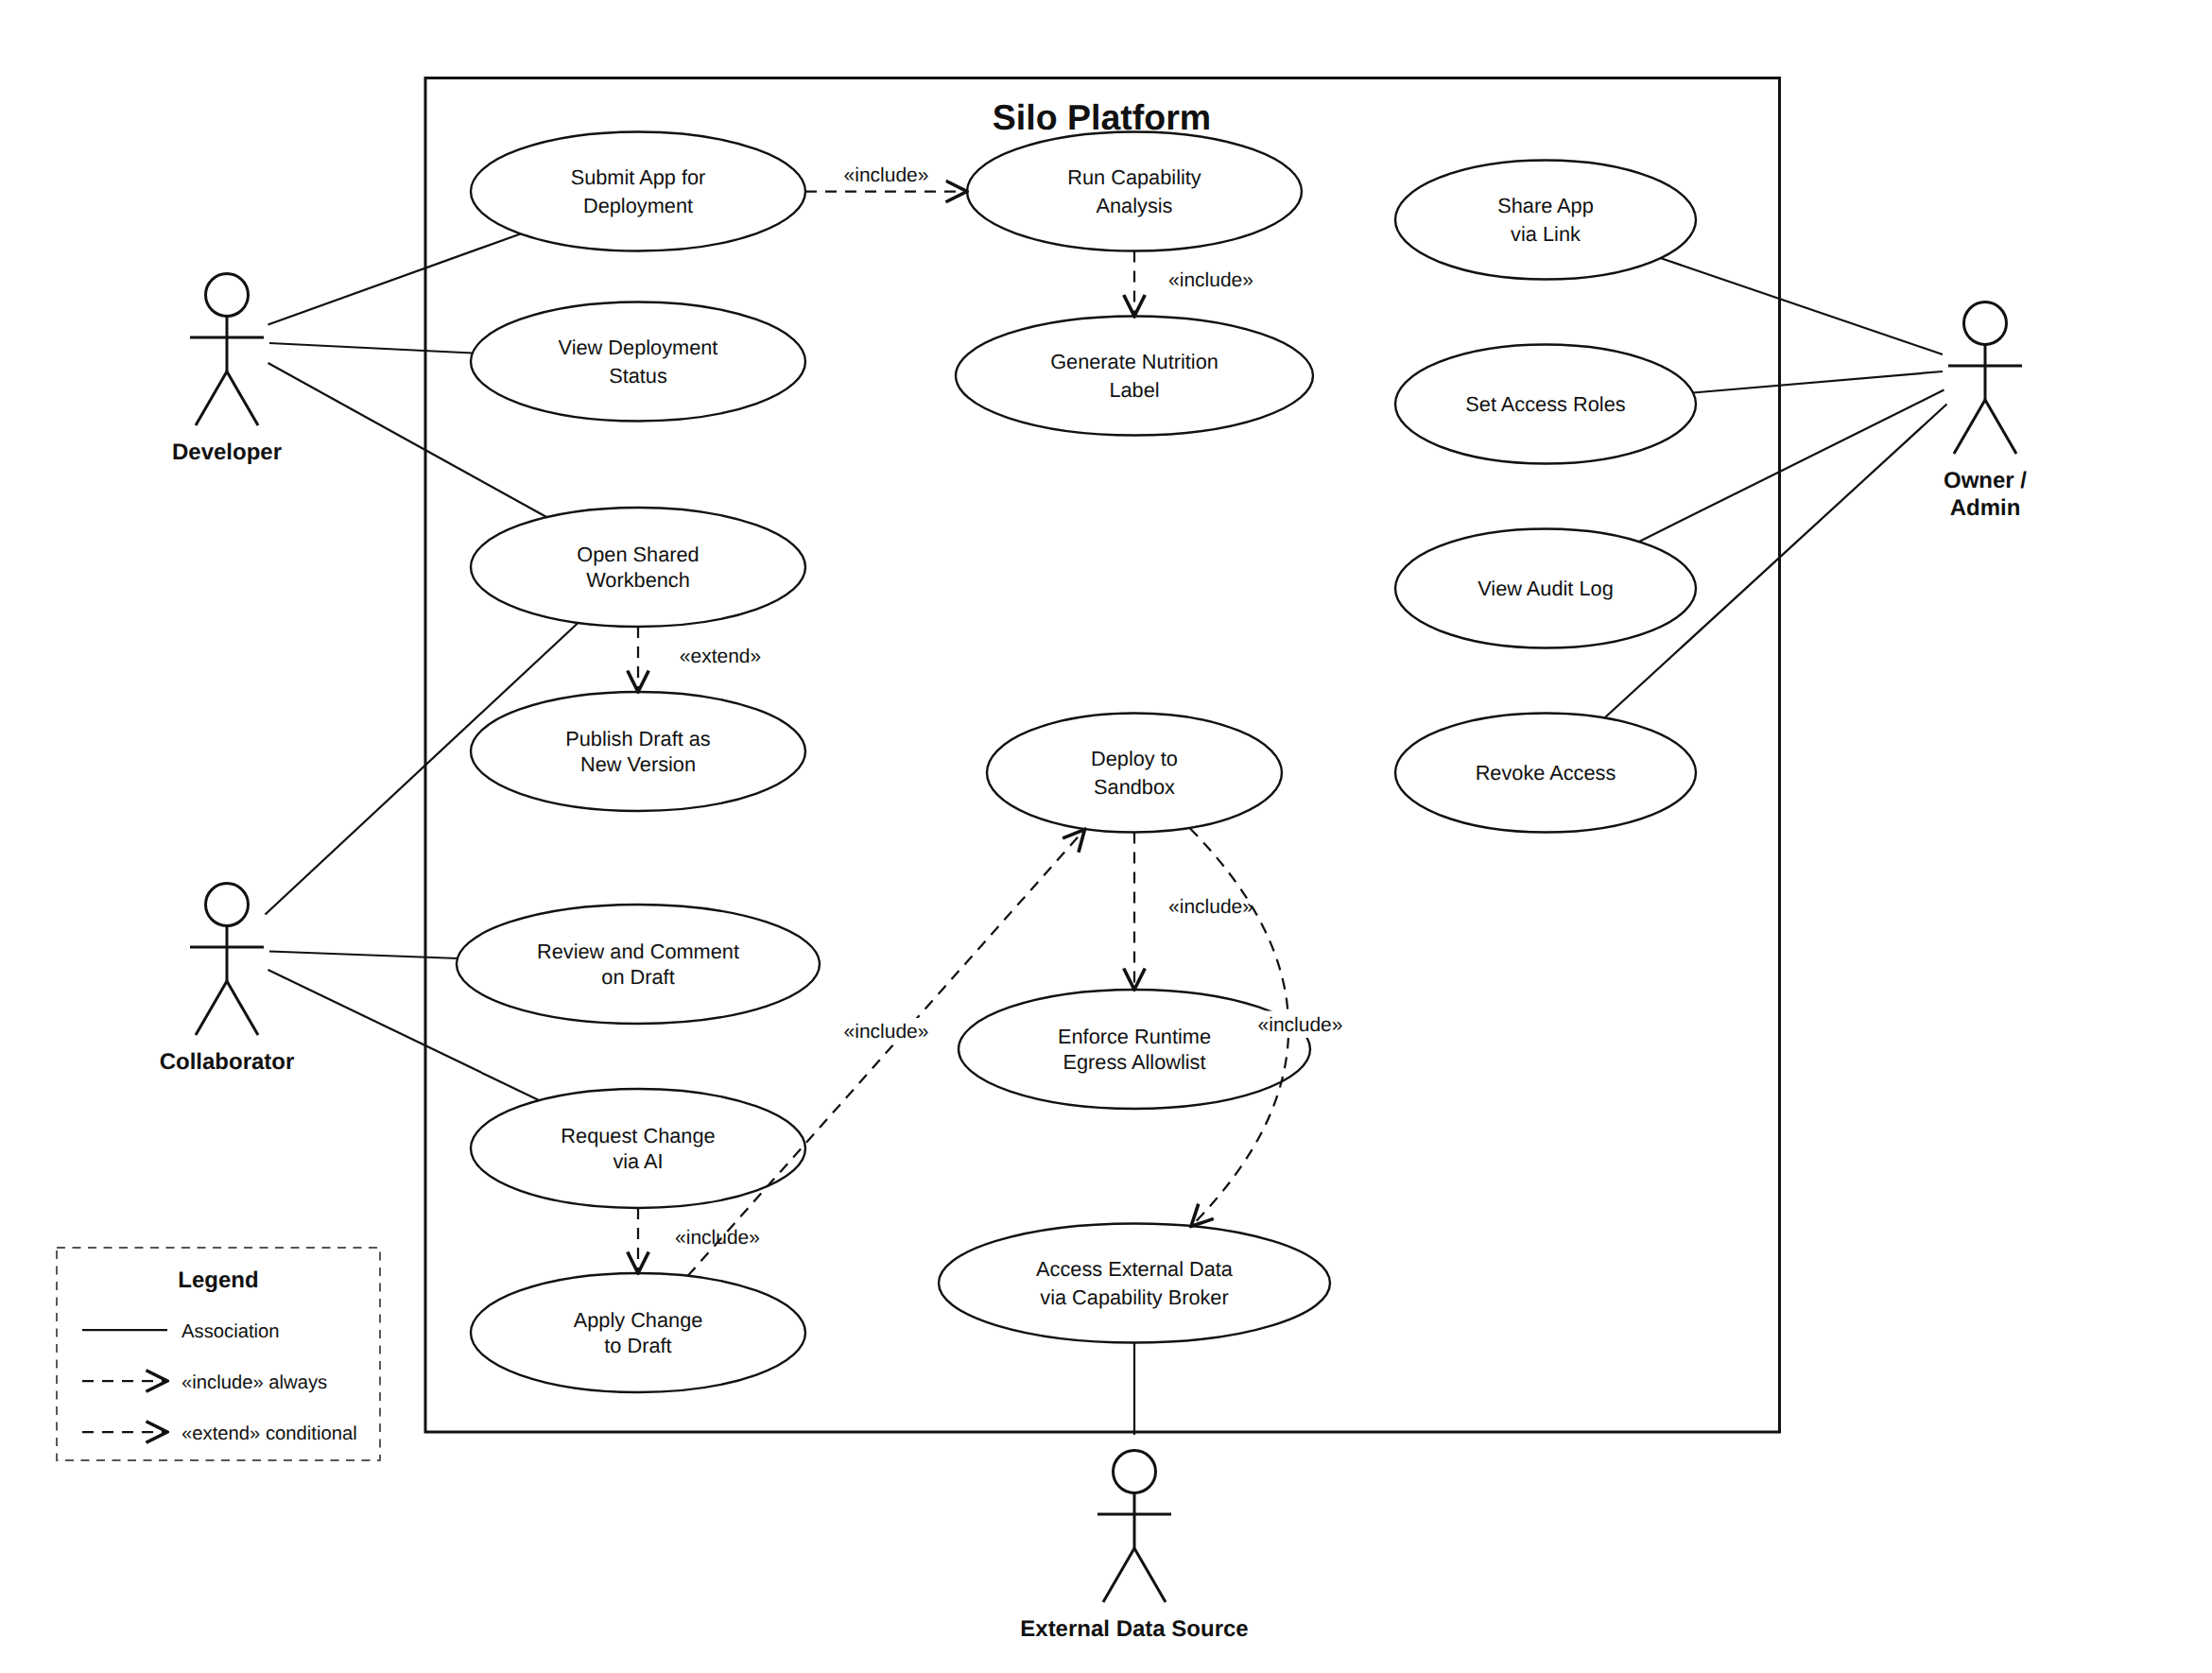
\includegraphics[width=\textwidth,height=0.62\textheight,keepaspectratio]{images/usecase.png}
  \caption{Use Case Diagram}
  \label{fig:usecase}
\end{figure}

\clearpage
\subsection{Activity Diagram}
\begin{figure}[H]
  \centering
  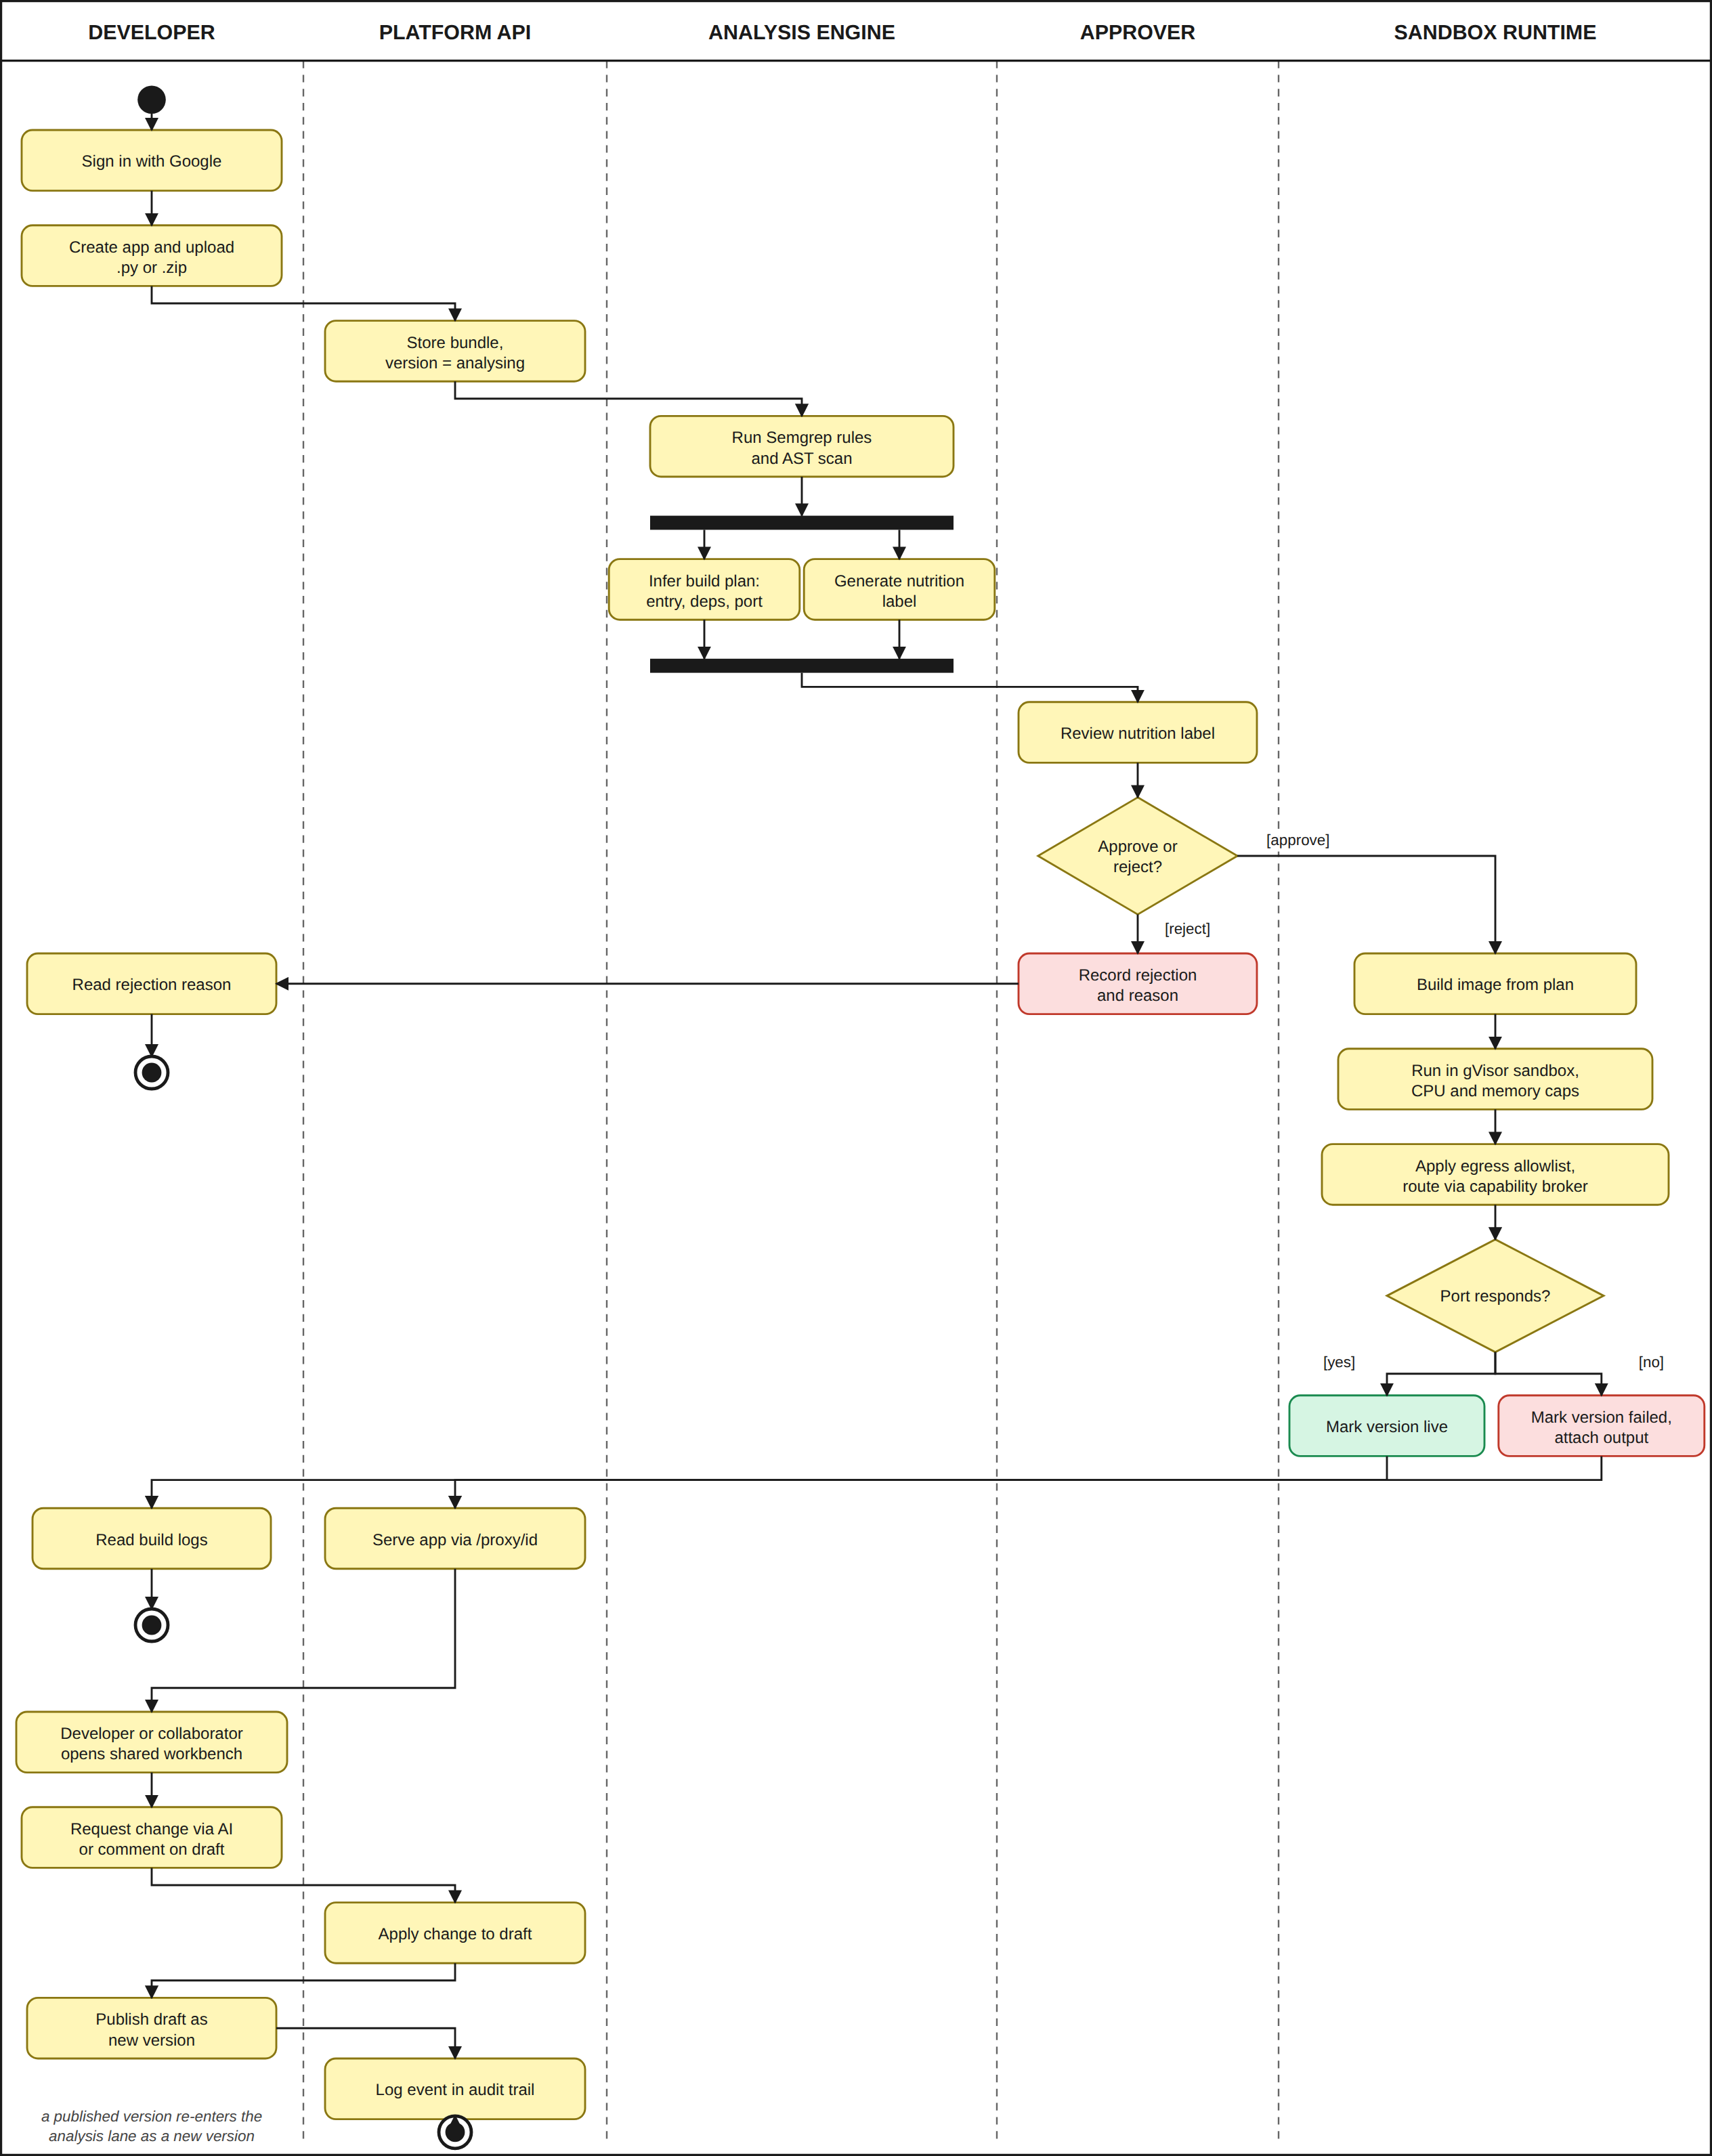
\includegraphics[width=\textwidth,height=0.68\textheight,keepaspectratio]{images/activity.png}
  \caption{Activity Diagram}
  \label{fig:activity}
\end{figure}

\clearpage
\subsection{Gantt Chart}
\begin{figure}[H]
  \centering
  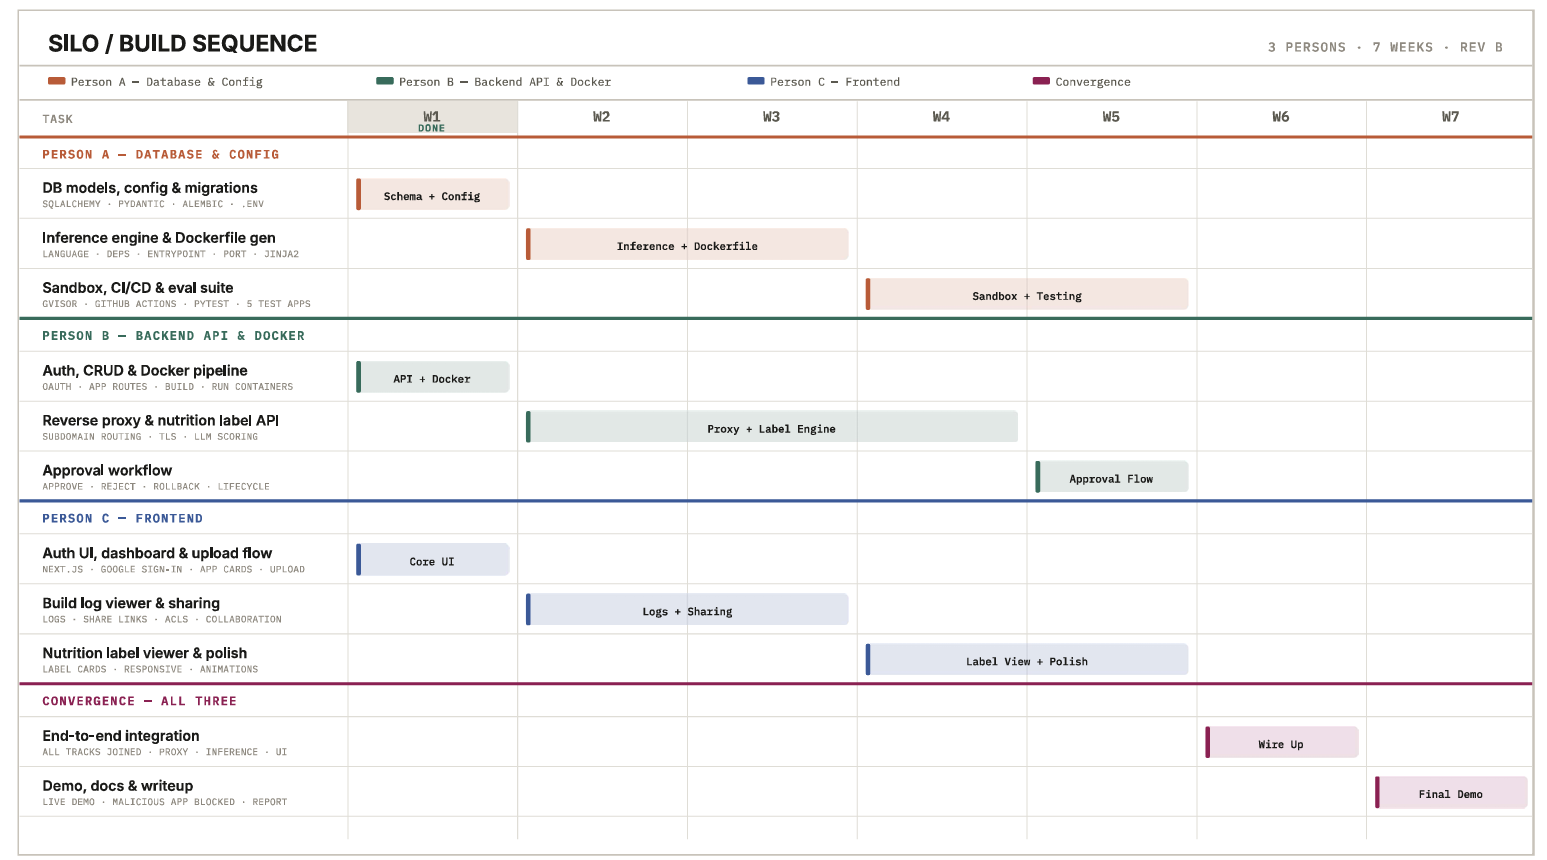
\includegraphics[width=\textwidth,height=0.68\textheight,keepaspectratio]{images/gantt.png}
  \caption{Gantt Chart}
  \label{fig:gantt}
\end{figure}

\clearpage
\subsection{Data Flow Diagram}
\begin{figure}[H]
  \centering
  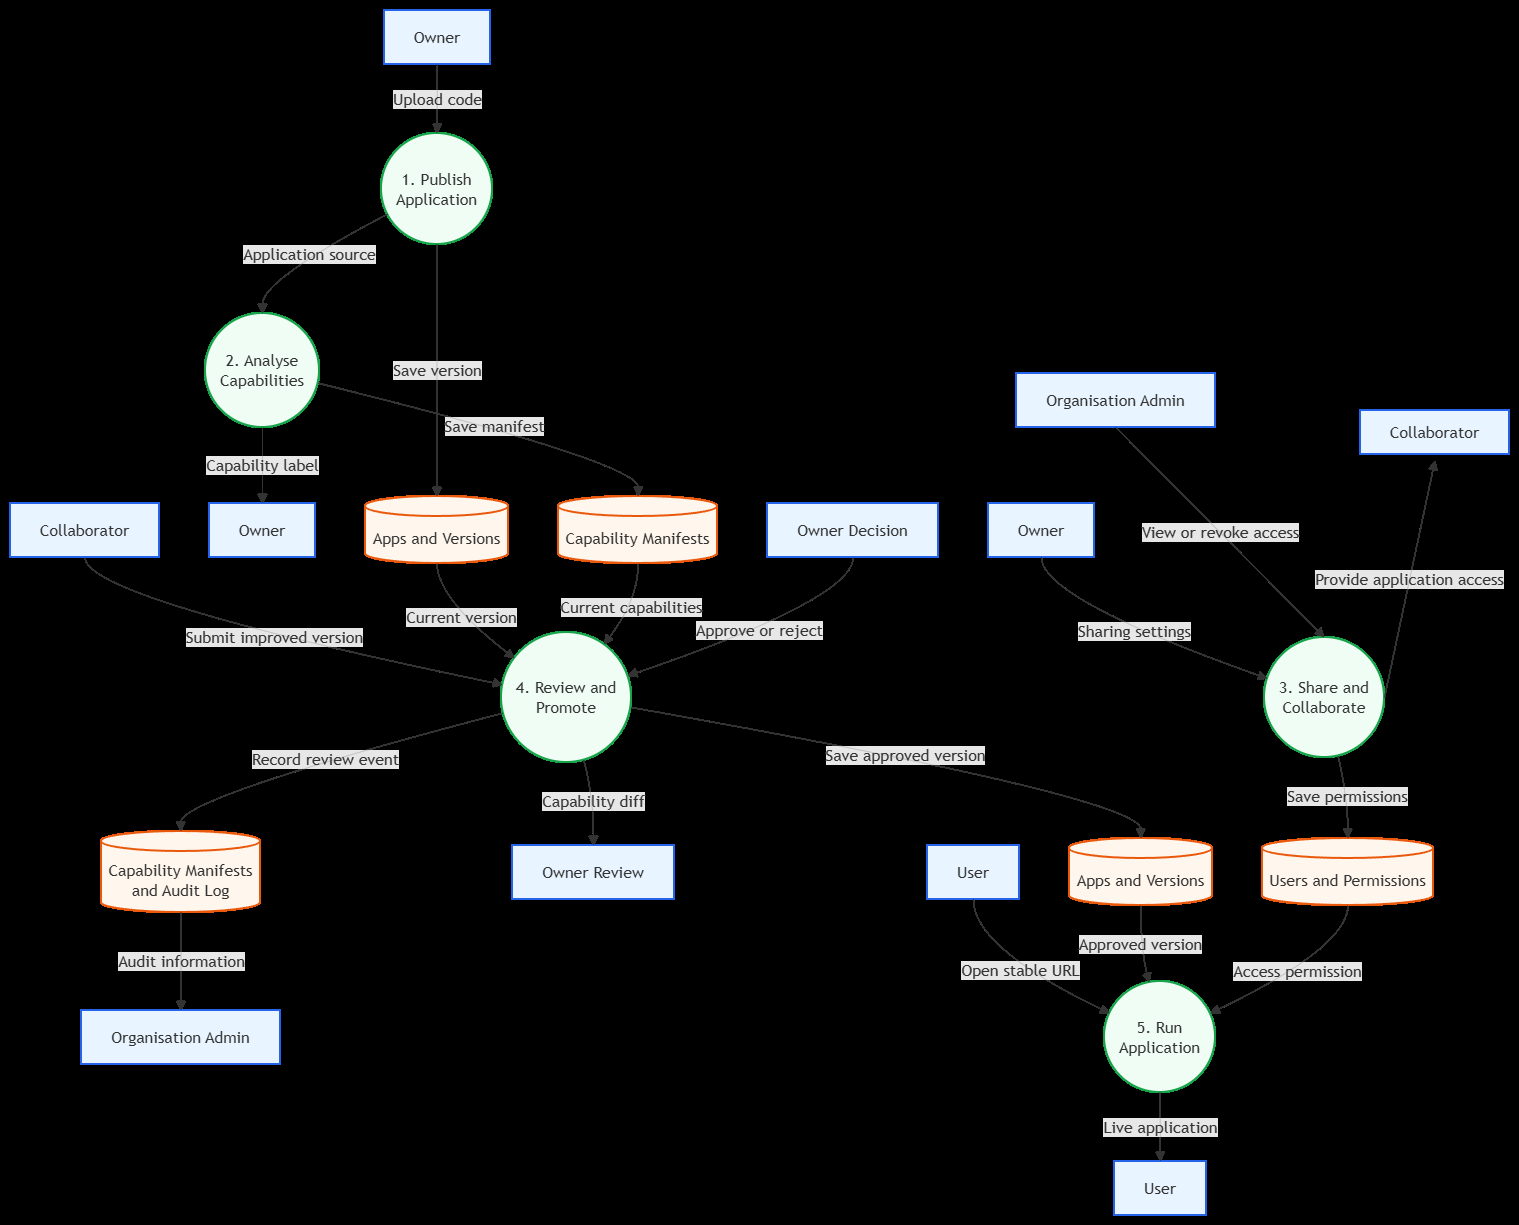
\includegraphics[width=\textwidth,height=0.68\textheight,keepaspectratio]{images/dataflow.png}
  \caption{Data Flow Diagram}
  \label{fig:dataflow}
\end{figure}

\clearpage
\subsection{Sequence Diagram}
\begin{figure}[H]
  \centering
  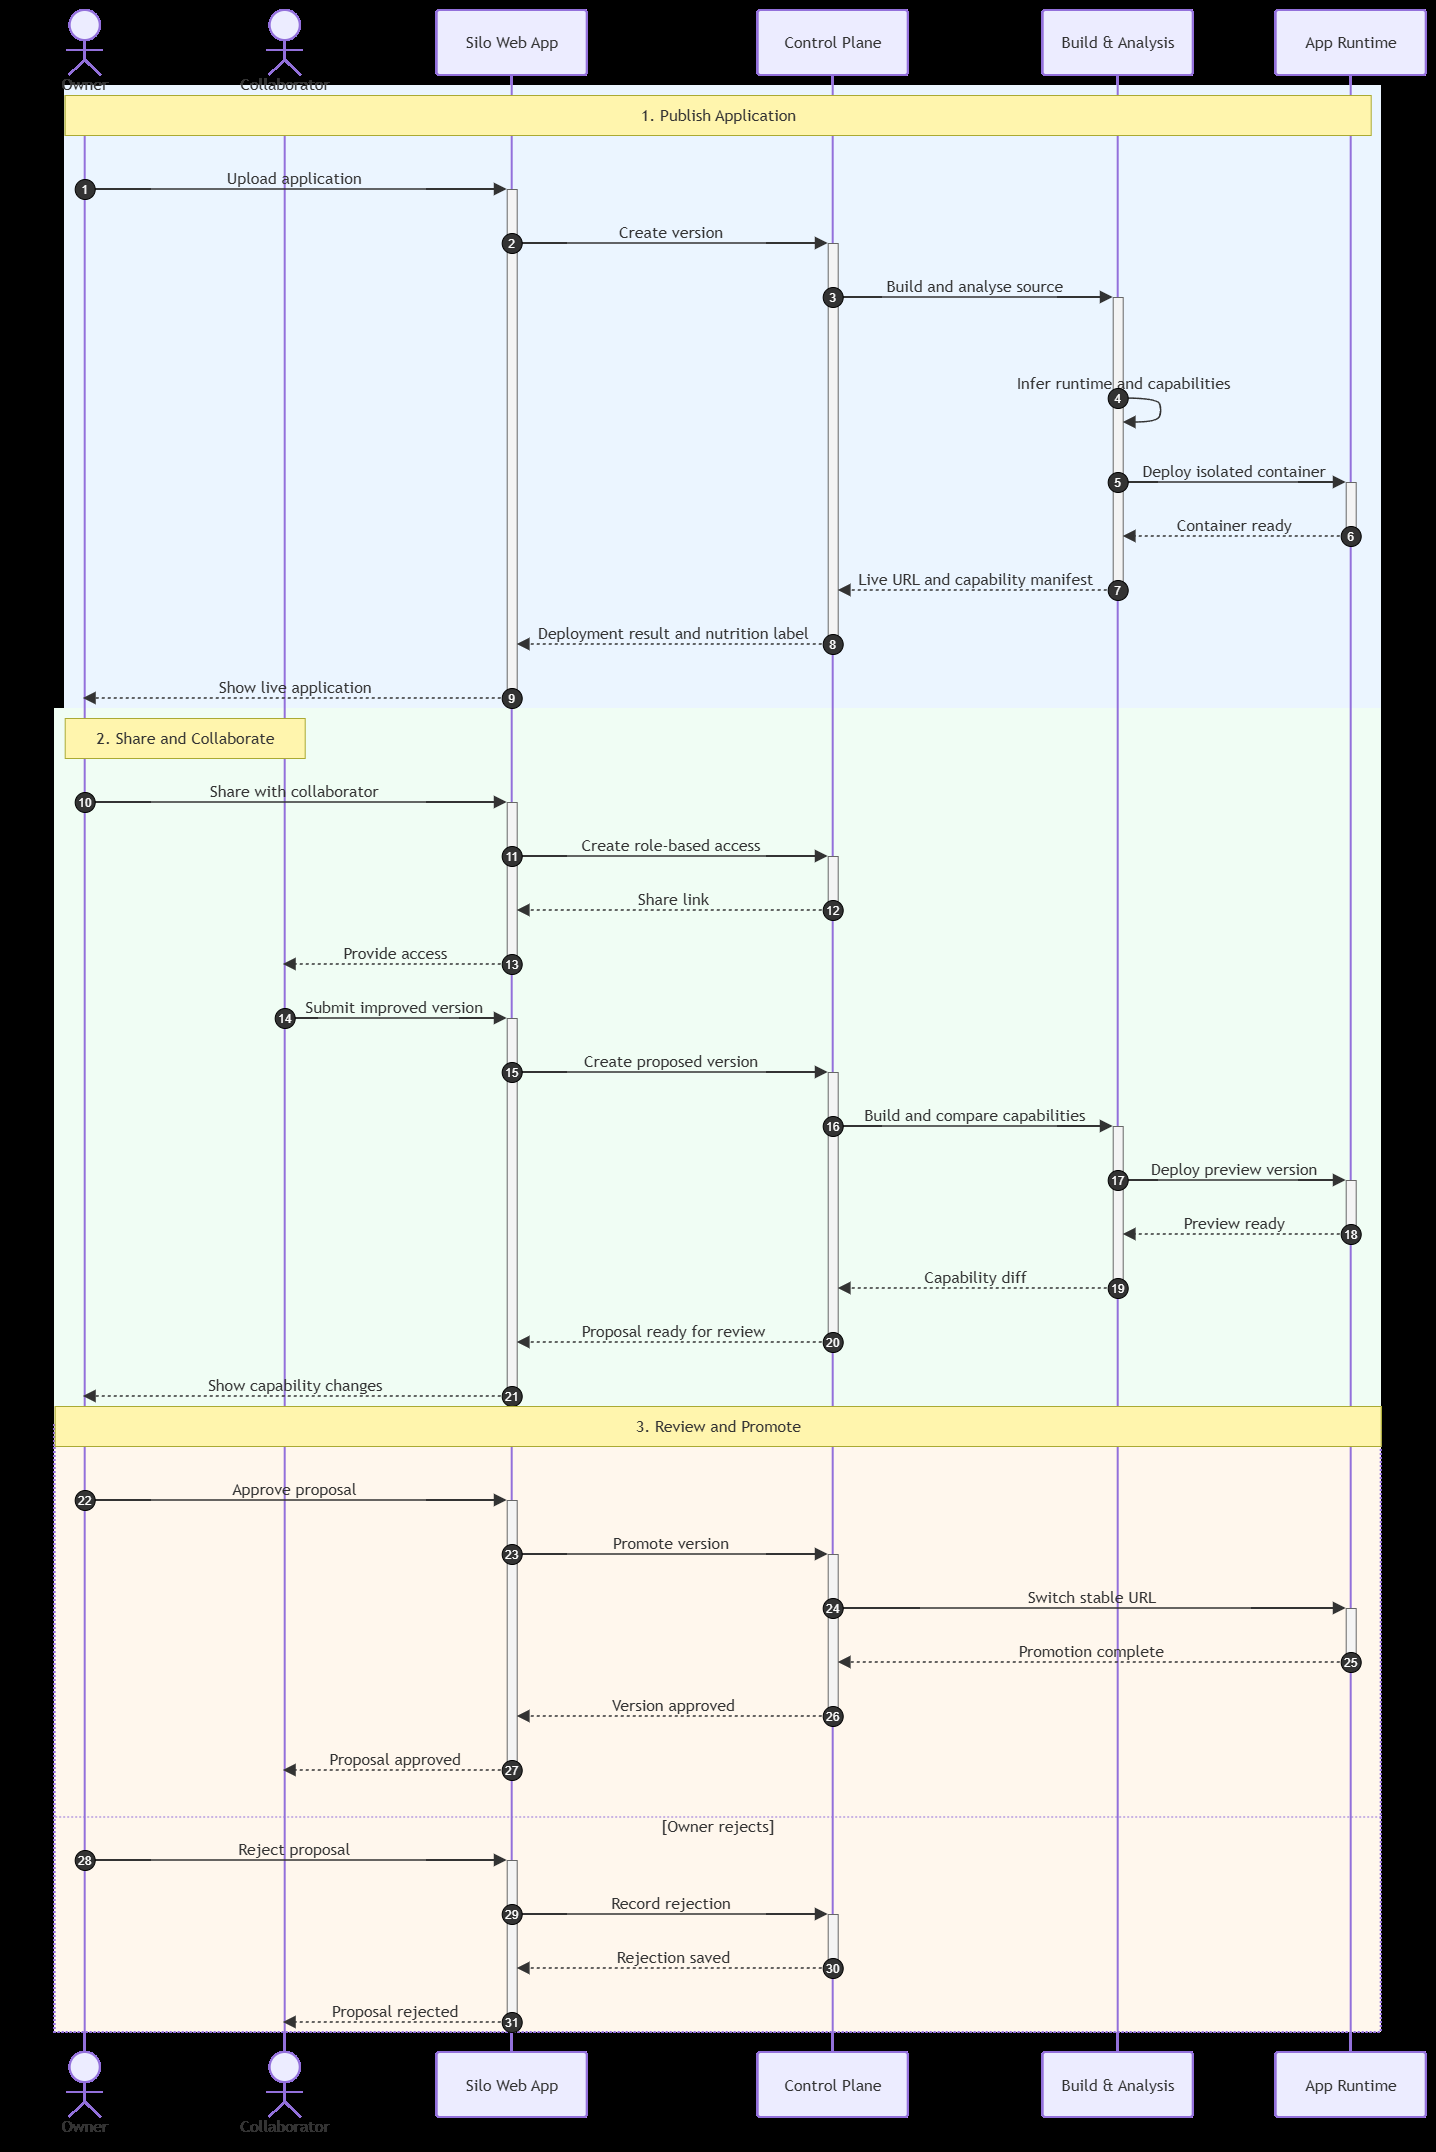
\includegraphics[width=\textwidth,height=0.68\textheight,keepaspectratio]{images/sequence.png}
  \caption{Sequence Diagram}
  \label{fig:sequence}
\end{figure}

\clearpage
\subsection{Collaboration Diagram}
\begin{figure}[H]
  \centering
  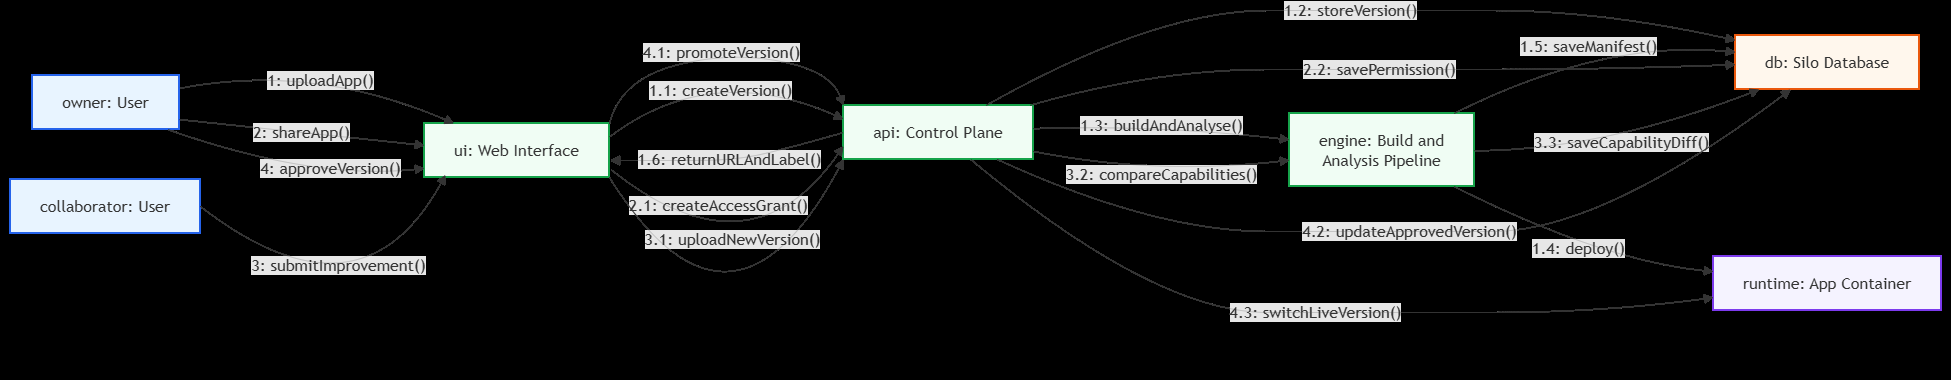
\includegraphics[width=\textwidth,height=0.68\textheight,keepaspectratio]{images/collaboration.png}
  \caption{Collaboration Diagram}
  \label{fig:collaboration}
\end{figure}

\clearpage
\subsection{Class Diagram}
\begin{figure}[H]
  \centering
  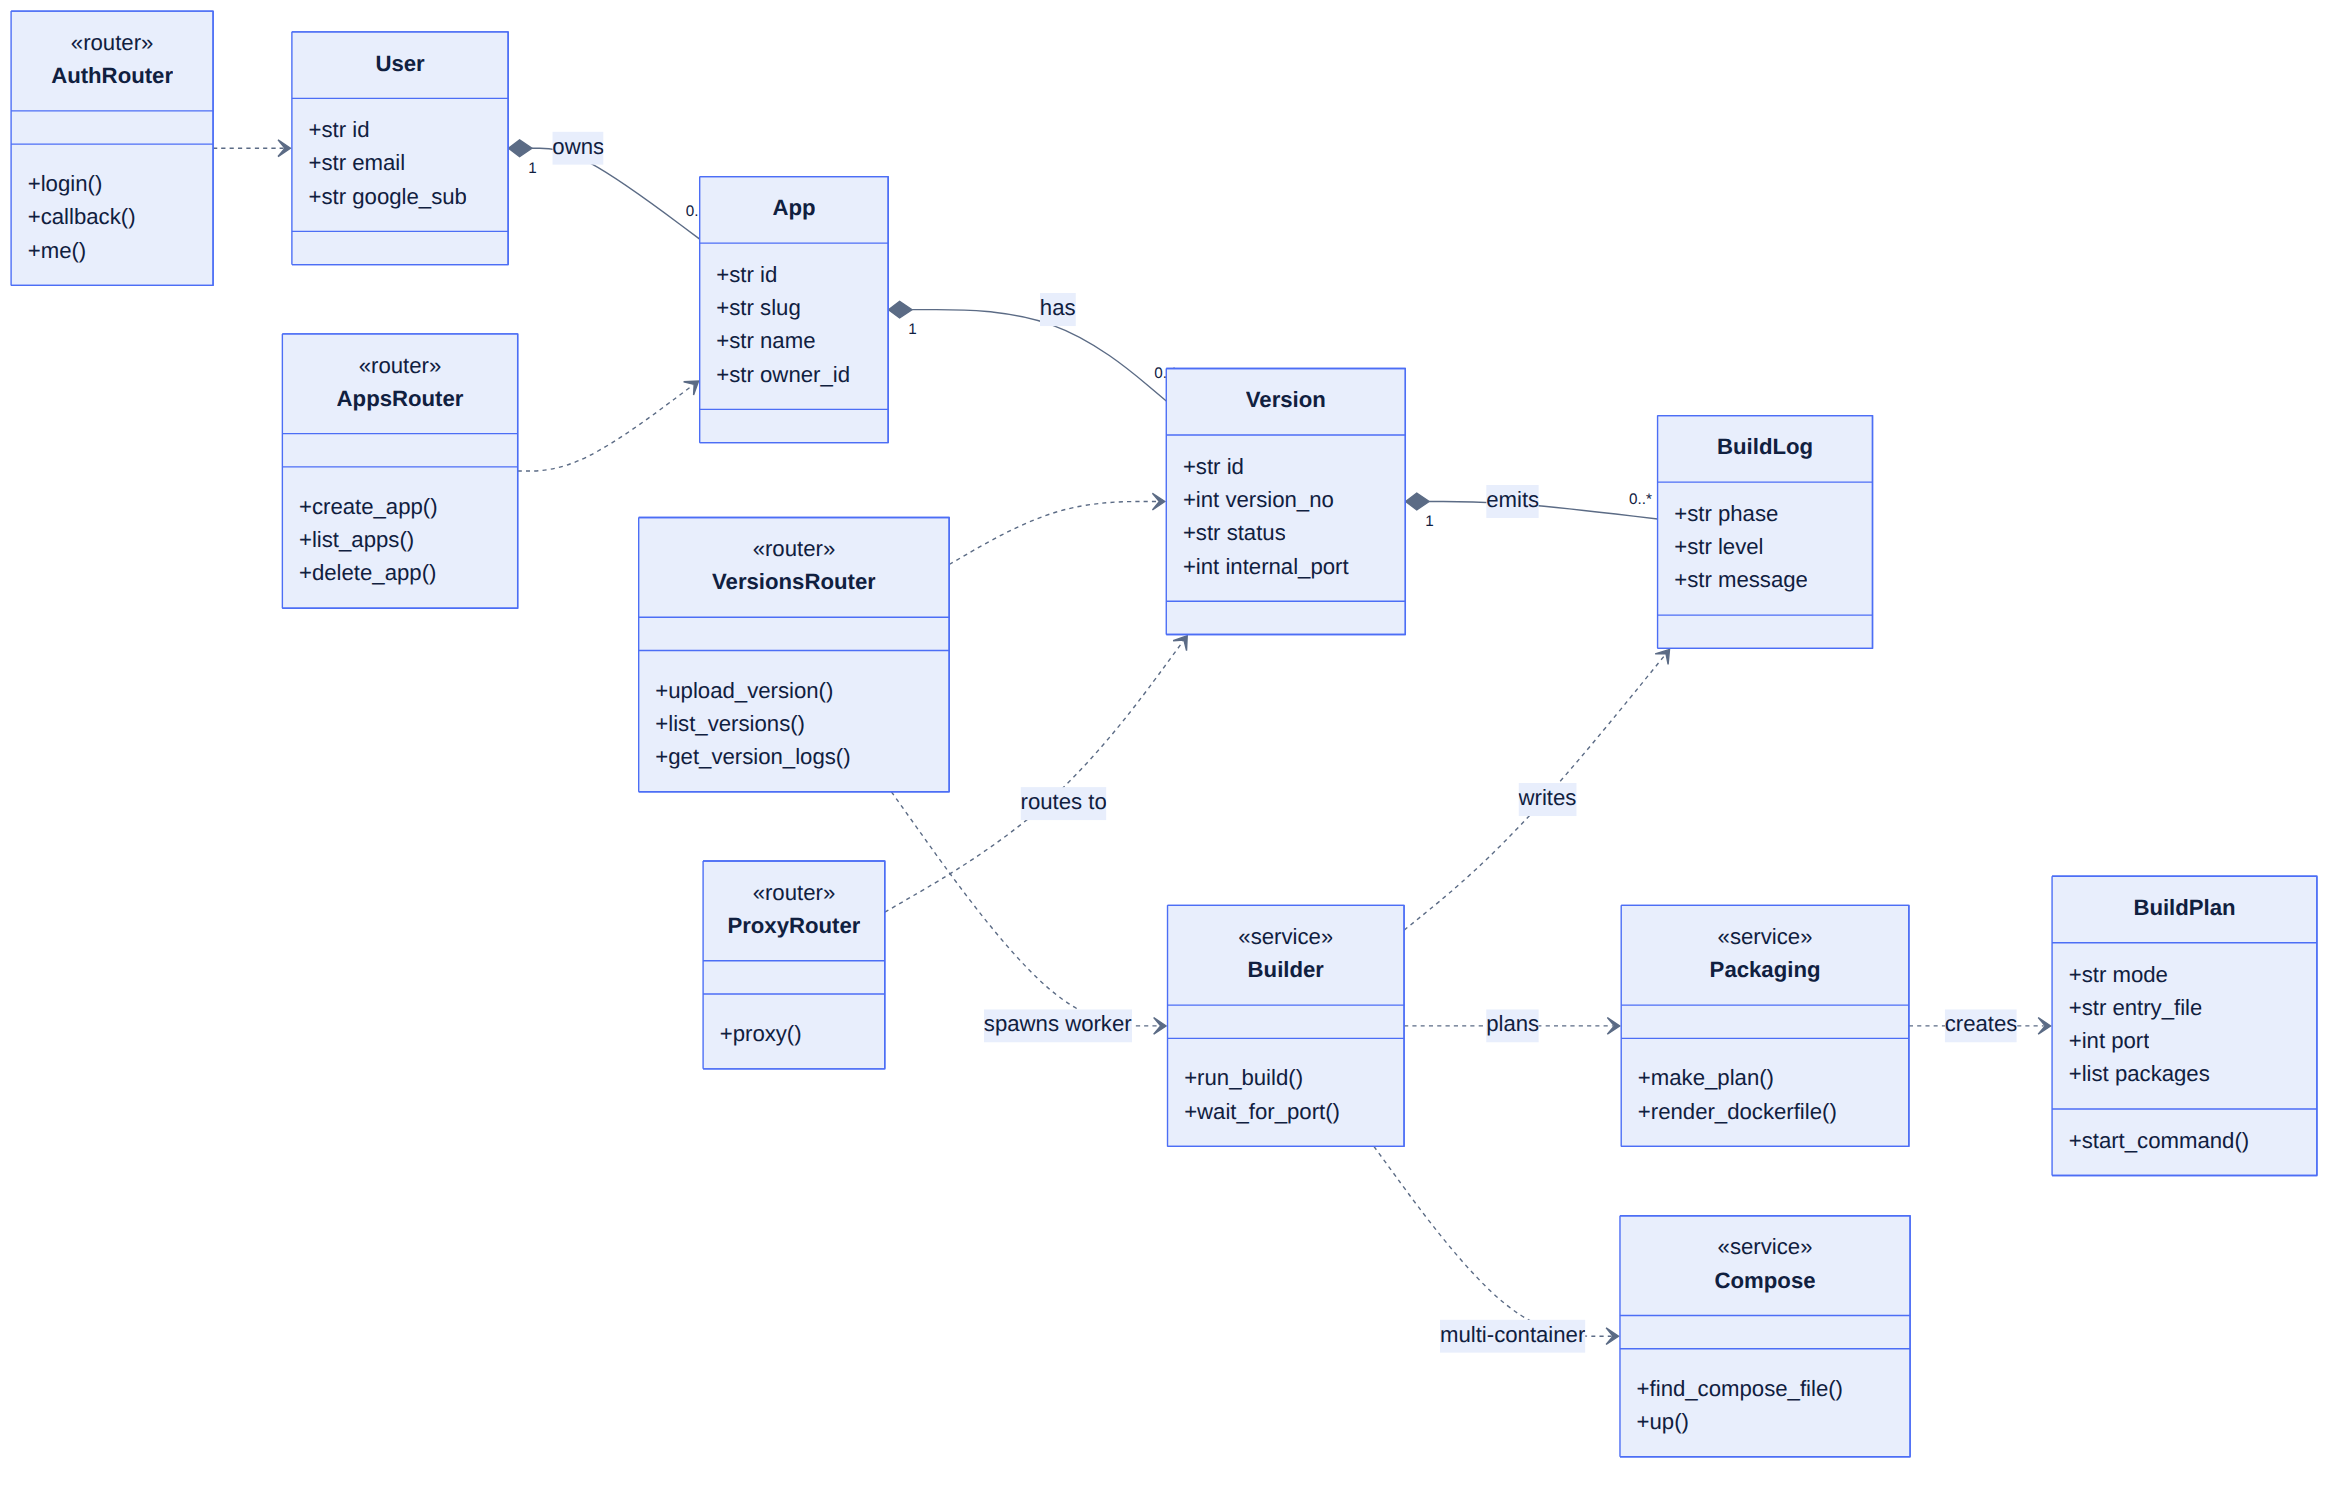
\includegraphics[width=\textwidth,height=0.68\textheight,keepaspectratio]{images/class.png}
  \caption{Class Diagram}
  \label{fig:class}
\end{figure}

\clearpage
\subsection{Use Case Specifications}
The following specification tables document the four primary operational use cases of the Silo platform:

\begin{figure}[H]
  \centering
  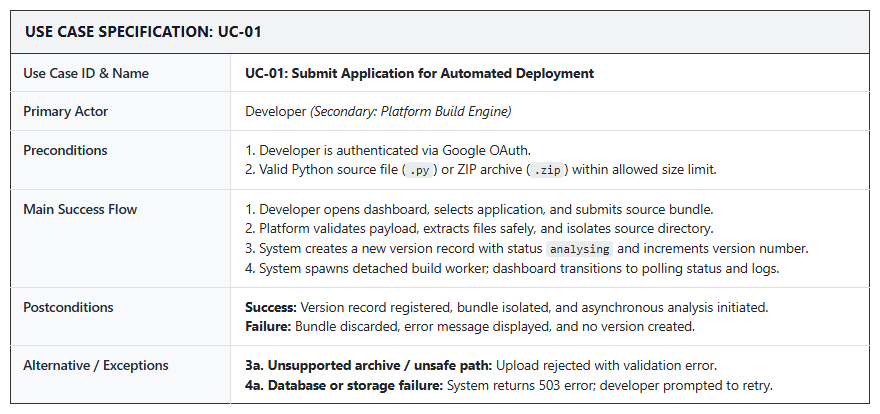
\includegraphics[width=0.92\textwidth]{images/usecase-template-1.png}
  \caption{Use Case Specification: UC-01 (Submit Application for Deployment)}
  \label{fig:uc-template-1}
\end{figure}

\begin{figure}[H]
  \centering
  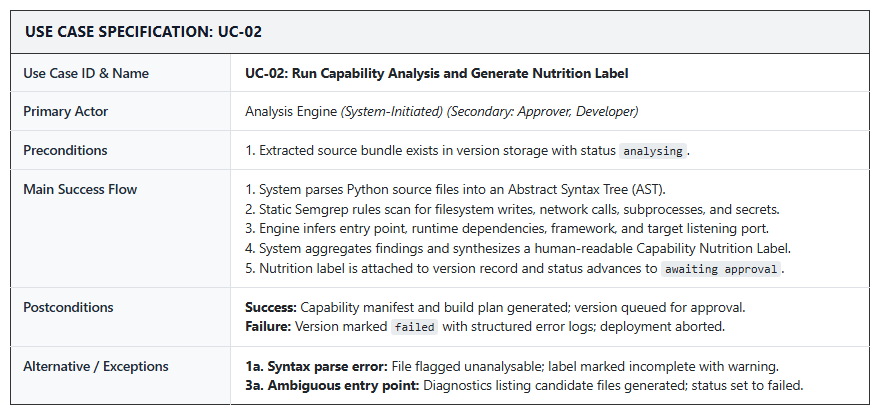
\includegraphics[width=0.92\textwidth]{images/usecase-template-2.png}
  \caption{Use Case Specification: UC-02 (Capability Analysis and Nutrition Label)}
  \label{fig:uc-template-2}
\end{figure}

\begin{figure}[H]
  \centering
  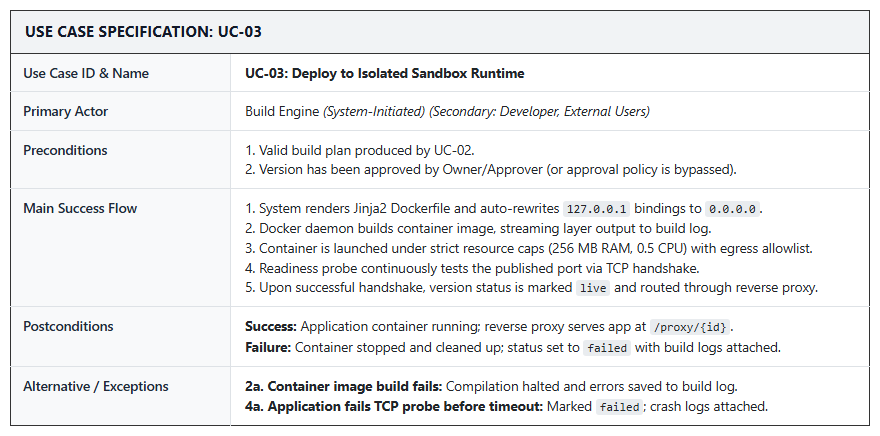
\includegraphics[width=0.92\textwidth]{images/usecase-template-3.png}
  \caption{Use Case Specification: UC-03 (Deploy to Isolated Sandbox)}
  \label{fig:uc-template-3}
\end{figure}

\begin{figure}[H]
  \centering
  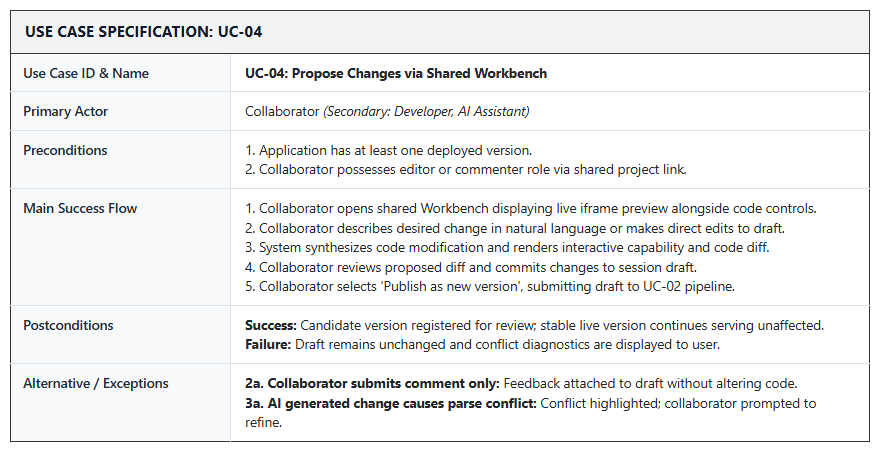
\includegraphics[width=0.92\textwidth]{images/usecase-template-4.png}
  \caption{Use Case Specification: UC-04 (Collaborative Workbench Change Request)}
  \label{fig:uc-template-4}
\end{figure}

\clearpage
\section{Implementation}

\subsection{Component Diagrams}
\begin{figure}[H]
  \centering
  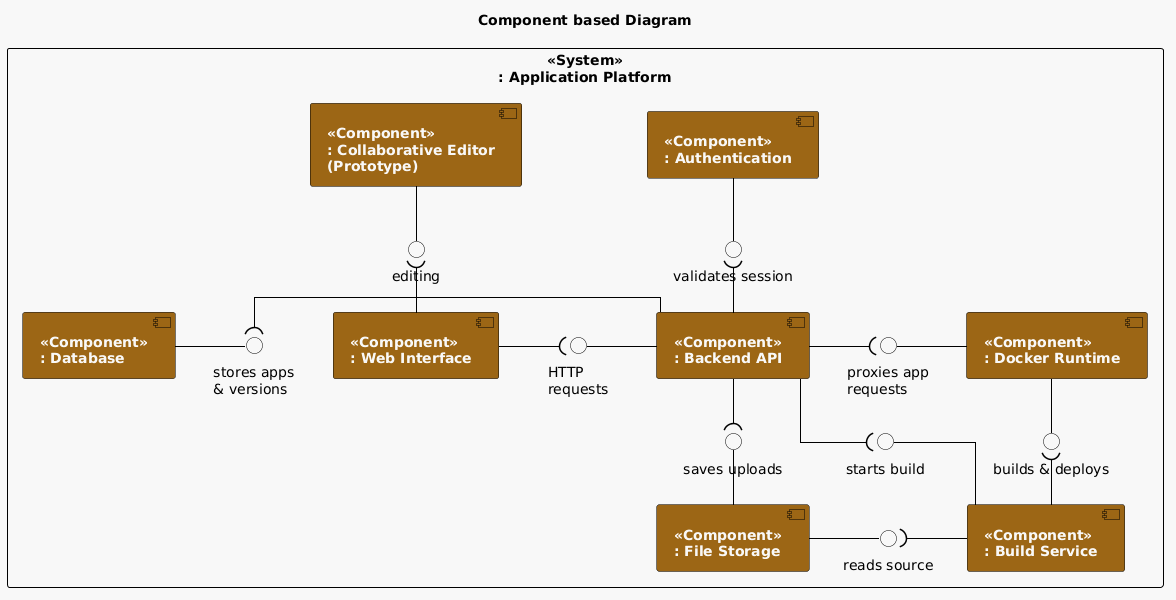
\includegraphics[width=\textwidth,height=0.62\textheight,keepaspectratio]{images/component.png}
  \caption{Component Diagram}
  \label{fig:component}
\end{figure}

\subsection{Deployment Diagrams}
\begin{figure}[H]
  \centering
  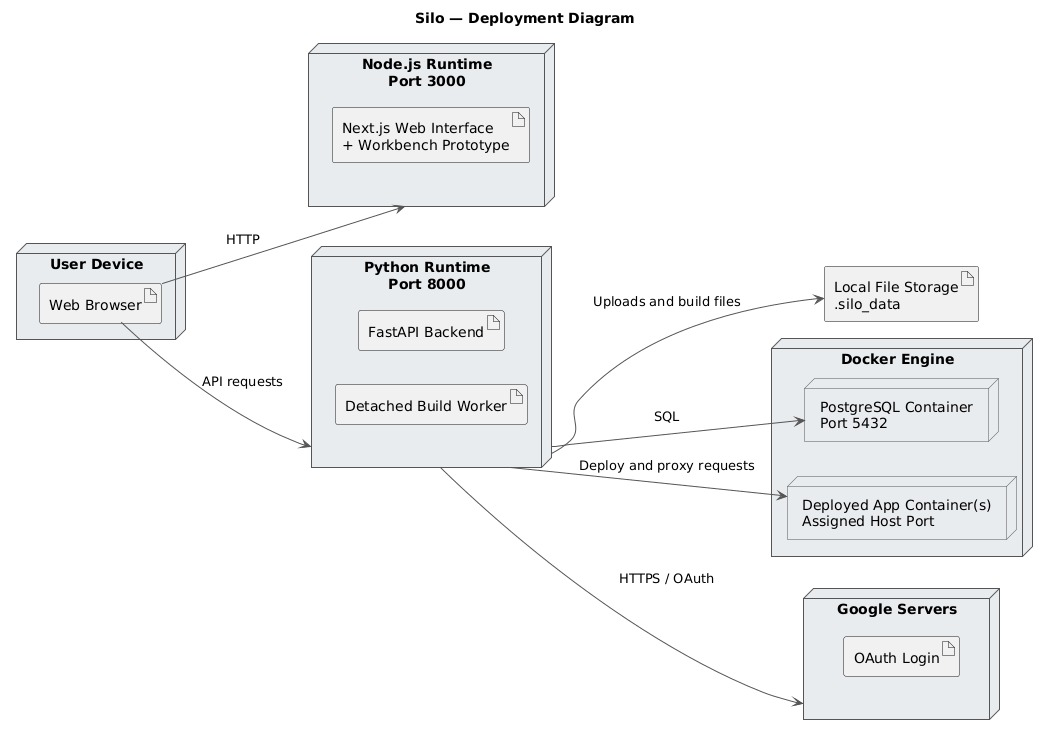
\includegraphics[width=\textwidth,height=0.62\textheight,keepaspectratio]{images/deployment.png}
  \caption{Deployment Diagram}
  \label{fig:deployment}
\end{figure}

\clearpage
\subsection{Screenshots}

\begin{figure}[H]
  \centering
  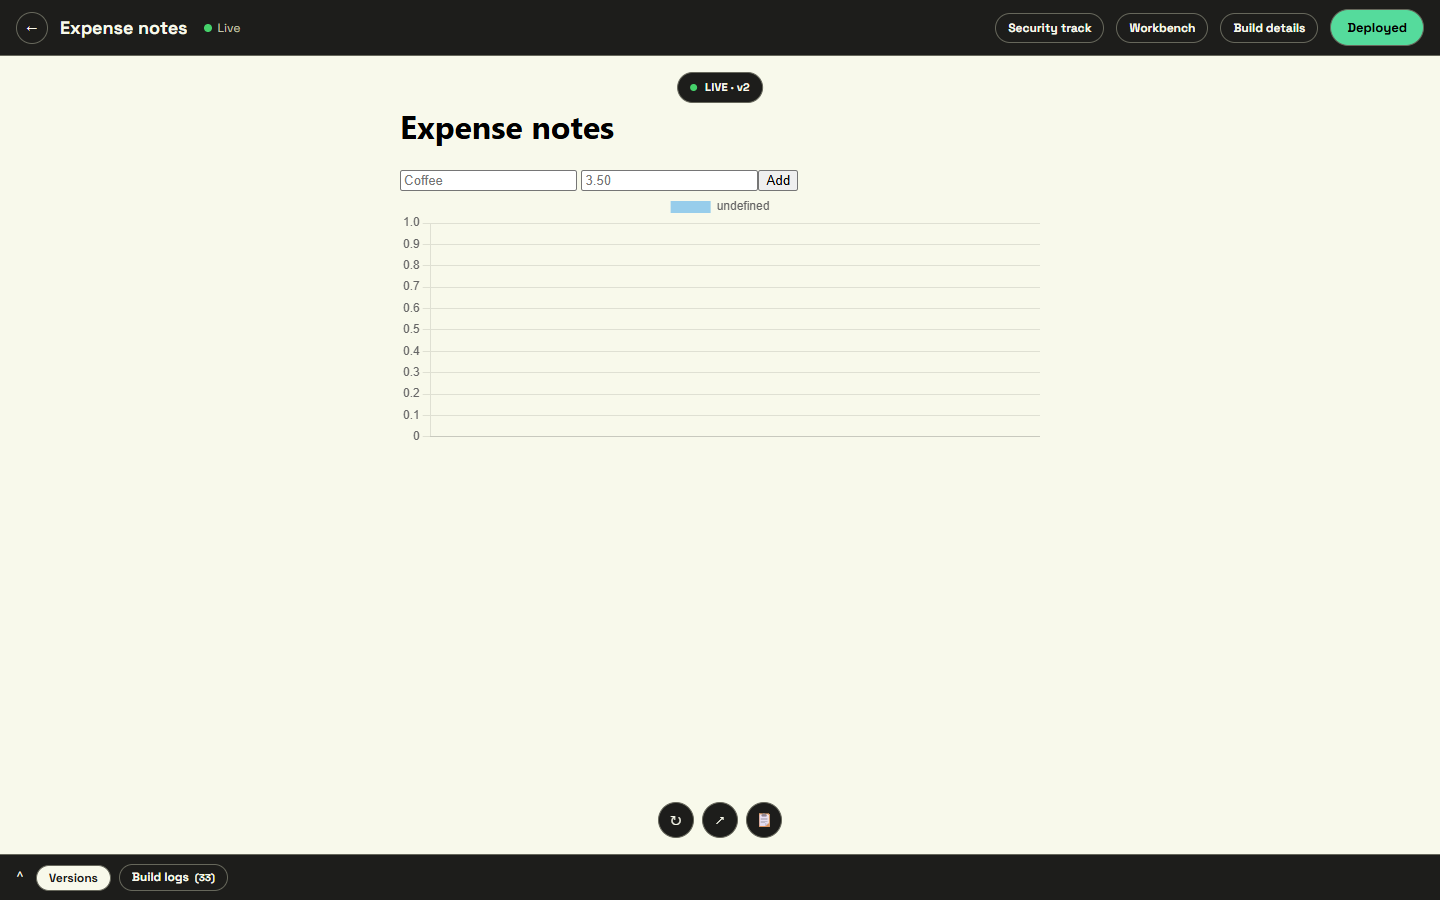
\includegraphics[width=0.95\textwidth]{images/ss-app-room.png}
  \caption{App Room: a Python app (Expense notes v2) running in Docker}
  \label{fig:ss-app-room}
\end{figure}

\begin{figure}[H]
  \centering
  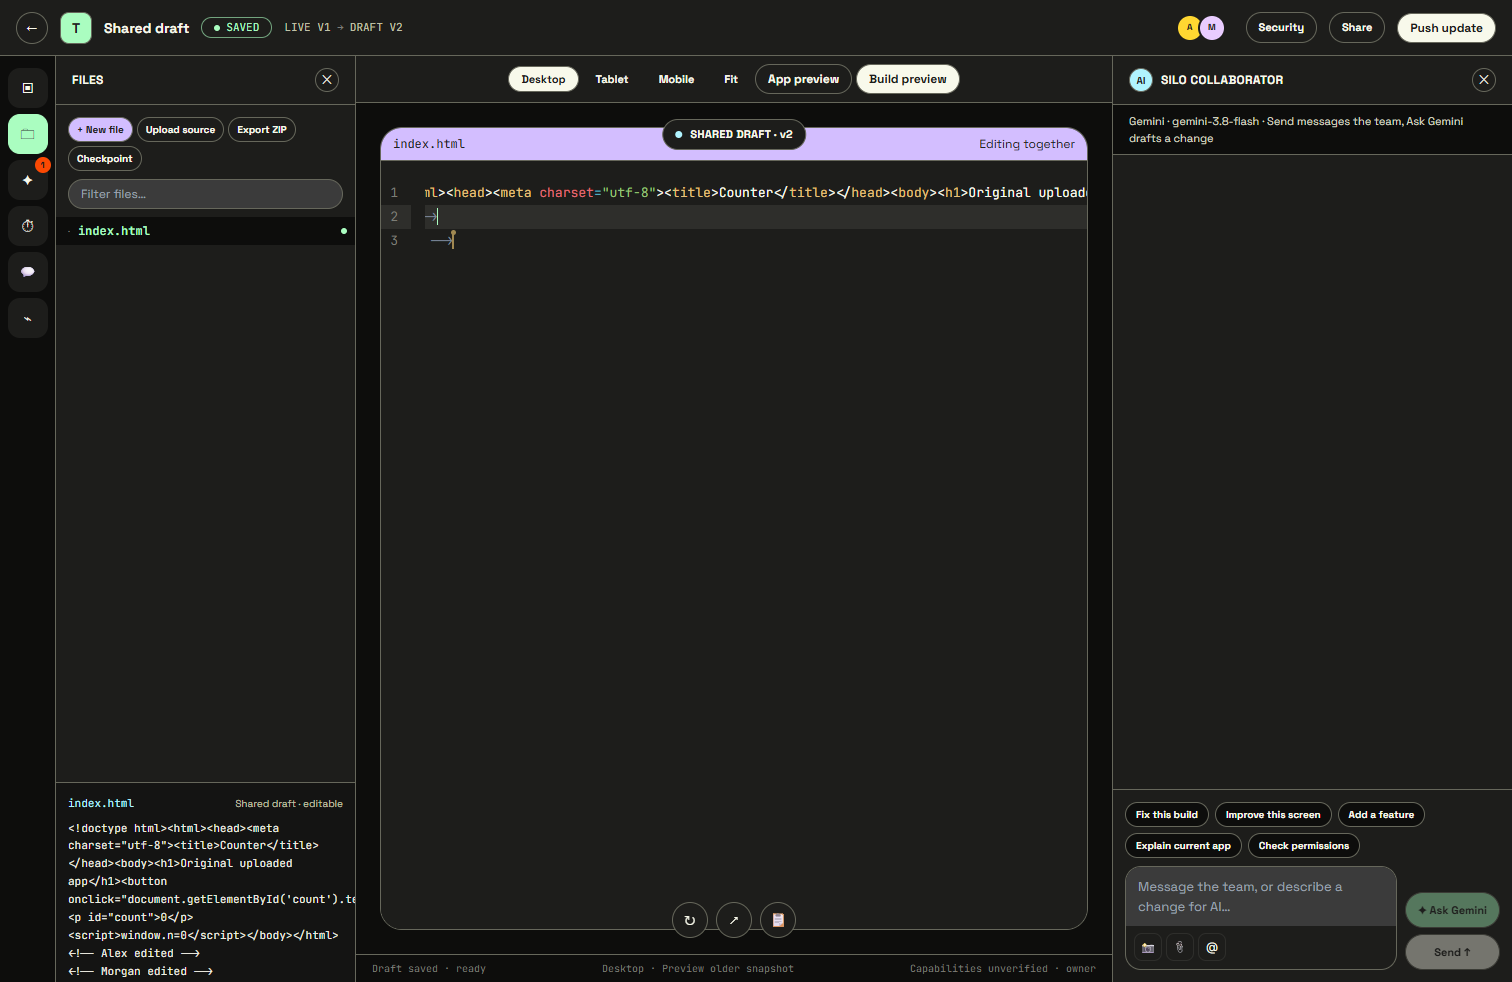
\includegraphics[width=0.95\textwidth]{images/ss-workbench.png}
  \caption{Workbench: two users' edits merged in the shared editor}
  \label{fig:ss-workbench}
\end{figure}

\begin{figure}[H]
  \centering
  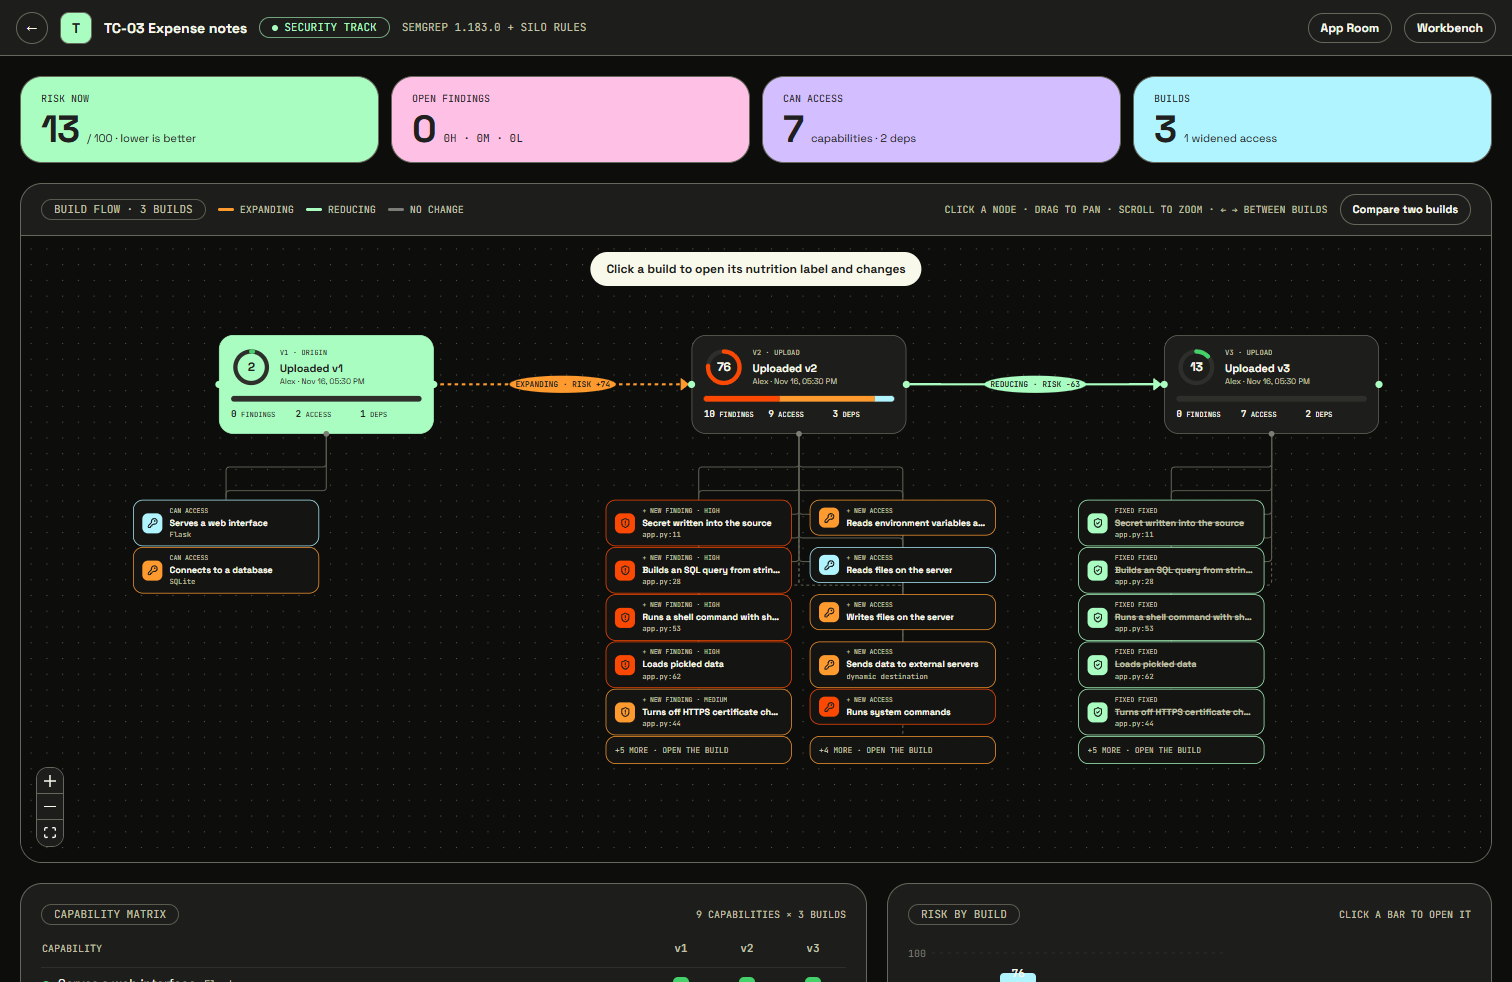
\includegraphics[width=0.95\textwidth]{images/ss-security-track.png}
  \caption{Security Track: three builds, Expanding then Reducing}
  \label{fig:ss-security-track}
\end{figure}

\flushbottom  % Restores original spacing behavior for the next chapters
% ===== CHAPTER 3: RESULTS & EVALUATION =====

\chapter{Results and Evaluation}

\section{Test Cases}
\raggedbottom  % test cases never split, so do not stretch the gaps between them

Four test cases were written in the course template and run on
17/11/2026. Each covers one of Silo's hardest promises.

\begin{table}[H]
\centering
\begin{tabular}{|l|p{6.2cm}|l|l|}
  \hline
  \textbf{ID} & \textbf{Test Case} & \textbf{Subsystem} & \textbf{Result} \\
  \hline
  TC-01 & Simultaneous editing & Workbench & Pass \\
  \hline
  TC-02 & Remove an editor during editing & Sharing and access & Pass \\
  \hline
  TC-03 & Security check of an update and its fix & Security Track & Pass \\
  \hline
  TC-04 & Detect hidden system commands & Security Track & Pass \\
  \hline
\end{tabular}
\caption{Test Case Summary}
\label{tab:testcases}
\end{table}

\TestCase{TC-01}{Simultaneous editing}{Workbench (shared editor)}{Deepank Agarwal}
{Test that two users editing the same line at the same time both keep their changes.}
{Alex (owner) and Morgan (editor) are logged in on separate computers. Both have the app ``Counter'' open in the Workbench, with \texttt{index.html} open.}
{1 & Both users click at the end of the last line of \texttt{index.html} & The cursor is placed at the end of the line on both screens & Pass & \\ \hline
 2 & At the same moment, Alex types `Alex edited' and Morgan types `Morgan edited' & Both lines appear on both screens; the status shows `Saving\ldots' then `Saved' & Pass & No error shown \\ \hline
 3 & Both users compare their screens & Both screens show the same text, each line once & Pass & \\ \hline
 4 & Morgan refreshes and opens \texttt{index.html} again & Both lines are still there & Pass & \\ \hline
 5 & \textbf{Check post-condition 1} & & Pass & \\ \hline}
{1. The saved file contains both lines, each exactly once.}

\TestCase{TC-02}{Remove an editor during editing}{Sharing and access}{Deepank Agarwal}
{Test that a removed editor loses access immediately, even with the editor still open.}
{Alex (owner) and Morgan (editor) are logged in; Morgan joined through an invitation link and has the Workbench open. Sam has an account but no access.}
{1 & Alex clicks `Share' and removes Morgan & Within 5 seconds, Morgan's screen shows `Access changed -- reload' & Pass & Shown after about 1 second \\ \hline
 2 & Morgan tries to type in the open file & The editor does not accept typing; nothing is saved & Pass & \\ \hline
 3 & Morgan refreshes the page & `App not found'; Morgan can no longer see the code & Pass & \\ \hline
 4 & Alex clicks `Revoke invitation links' & The message `Invitation links revoked' appears & Pass & \\ \hline
 5 & Sam opens the old invitation link & `Invitation not found' is displayed & Pass & \\ \hline
 6 & \textbf{Check post-condition 1} & & Pass & \\ \hline}
{1. Morgan is removed from the app's member list; only Alex remains.}

\TestCase{TC-03}{Security check of an update and its fix}{Security Track}{Pushti}
{Test that the Security Track finds the problems a new version adds and recognises when they are fixed.}
{Alex is logged in with an empty app ``Expense notes''. Three versions are ready: v1 (safe), v2 (10 known security problems), v3 (v2 with all 10 fixed).}
{1 & Upload v1, then v2, then v3 & Three versions are shown & Pass & \\ \hline
 2 & Open the Security Track & v1$\to$v2 marked `Expanding', v2$\to$v3 marked `Reducing' & Pass & \\ \hline
 3 & Click v1 & Label: serves a web page, uses a database; no problems & Pass & \\ \hline
 4 & Click v2 & 10 problems (4 high, 5 medium, 1 low), high risk score & Pass & Risk 76 of 100 \\ \hline
 5 & Open the list of problems for v2 & Each shows where it is and how to fix it; the secret key is not displayed & Pass & \\ \hline
 6 & Click v3 & No problems; the 10 listed as fixed; risk drops & Pass & Risk 13 of 100 \\ \hline
 7 & \textbf{Check post-condition 1} & & Pass & \\ \hline}
{1. The risk chart shows one bar for each of the three versions.}

\TestCase{TC-04}{Detect hidden system commands}{Security Track}{Simar Verma}
{Test that the Security Track detects an app that runs system commands even when the code hides it.}
{Alex is logged in with an empty app. Two versions are ready: v1 (safe) and v2 (adds a hidden admin page that runs any command sent to it, with the commands disguised in the code).}
{1 & Upload v1, then v2 & Two versions are shown & Pass & \\ \hline
 2 & Open the Security Track and click v2 & v1$\to$v2 is marked `Expanding' & Pass & \\ \hline
 3 & Open the label for v2 & The label lists `Runs system commands' & Pass & \\ \hline
 4 & Open the list of problems for v2 & A high-severity problem for each hidden command & Pass & All 3 commands found \\ \hline
 5 & Look for a warning about the disguised code & A warning that the code hides which part of the program it loads & Pass & \\ \hline
 6 & \textbf{Check post-condition 1} & & Pass & \\ \hline}
{1. v2's risk score is higher than v1's.}

\flushbottom
\section{Analysis}

\begin{itemize}

  \item \textbf{Objectives met.} All four test cases pass. The
  automated suites also pass: 117 API tests, 9 browser tests
  (including the four test cases) and 2 collaboration tests, with
  clean lint and type checks.

  \item \textbf{Key results.} Concurrent edits merged with no loss or
  duplication (TC-01). A removed editor was cut off in about 1 second
  against a 5-second target (TC-02). The Security Track found all 10
  planted problems, with the risk falling from 76 to 13 after the fix
  (TC-03).

  \item \textbf{Improvement found through testing.} TC-04 first
  failed: the analyser matched function names only as written, so
  commands hidden behind renamed imports, \texttt{importlib},
  \texttt{\_\_import\_\_} or \texttt{getattr} were missed (risk 12, one
  finding). A name resolver was added that traces each call to its real
  function. The test then passed (risk 41, all three commands found),
  and regression tests now protect the fix.

  \item \textbf{Limitations.} The Security Track is static analysis: it
  narrows risk but cannot prove an app safe. Collaboration uses one
  server per installation, workspaces are limited to 150 text files
  (3\,MB), and the local AI handles projects up to about 24,000
  characters before falling back to Gemini.

\end{itemize}

\FloatBarrier

% ===== CHAPTER 4: CONCLUSION =====

\chapter{Conclusion}

\section{Summary of Work}

The finished system delivers the full ``Google Docs for small
software'' workflow:

\begin{enumerate}

  \item Zero-configuration deployment of static and Python apps, with
  Compose, Dockerfile and generated-image strategies and a real
  readiness check.

  \item Real-time collaborative editing with comments, chat,
  checkpoints, previews and publishing.

  \item Role-based sharing with revocable invitation links and
  immediate loss of access on removal.

  \item The Security Track: rule-based capability labels, findings,
  version comparison and risk scores, shown as an interactive flow.

  \item An AI collaborator that proposes reviewable changes, running
  locally on the GPU with Gemini as the fallback.

  \item One-command local hosting and automated tests at every level.

\end{enumerate}


\section{Key Findings}

\begin{itemize}

  \item \textbf{Deterministic rules are enough to deploy and audit
  small apps.} Neither deployment nor security decisions need a
  language model, which keeps them fast and explainable.

  \item \textbf{``Running'' is not ``ready''.} Only a real HTTP
  response proves that a deployment works.

  \item \textbf{The database must stay the source of truth.} Saving
  each edit before confirming it, and re-checking roles on every save,
  made collaboration both safe and reliable.

  \item \textbf{Hard test cases improve the product.} TC-04 exposed a
  real blind spot in the analyser that was then fixed.

  \item \textbf{A small local model is practical} when its output is
  constrained to a schema and always reviewed by a person.

\end{itemize}


\section{Future Work and Recommendations}

\begin{enumerate}

  \item Stronger runtime isolation (gVisor) and network egress limits
  for uploaded apps.

  \item Scale-to-zero for idle containers.

  \item Node.js application support.

  \item Several collaboration servers for larger teams.

  \item A user study with non-expert participants on the nutrition
  label and review flow.

\end{enumerate}


\section{Final Remarks}

Silo began with a simple observation: generating code is easy, but
turning it into a shared, trustworthy application is not. The finished
system lets a team upload an app, run it with no configuration, improve
it together in real time, and see exactly what each new version can do
before trusting it.


% ===== BIBLIOGRAPHY =====

% Print bibliography with heading in TOC
\printbibliography[heading=bibintoc]

\end{document}
